\documentclass[12pt,a4paper]{article}

% Packages
\usepackage[utf8]{inputenc}
\usepackage{dirtree}
\usepackage{amsmath}
\usepackage{amssymb}
\usepackage{graphicx}
\usepackage{hyperref}
\usepackage{geometry}
\usepackage{cleveref}
\usepackage{enumitem}
\usepackage{booktabs}

\geometry{a4paper, margin=1in}

% Title Page
\title{Dysruption - Action Analysis}
\author{Rishitosh Kumar Singh}
\date{\today}

\begin{document}

\maketitle

\section{Introduction}
\label{sec:introduction}
    This report presents the work done over the semester on a project focused on analyzing decision-making strategies within critical infrastructure networks through interactive simulation games. The main objective was to design and develop bots that could autonomously play two online strategy games—\textit{Break it Bad} and \textit{Save Our System (Scenario 1)} and evaluate their performance by recording and analyzing their actions and corresponding scores.

    \begin{figure}[h!]
        \centering
        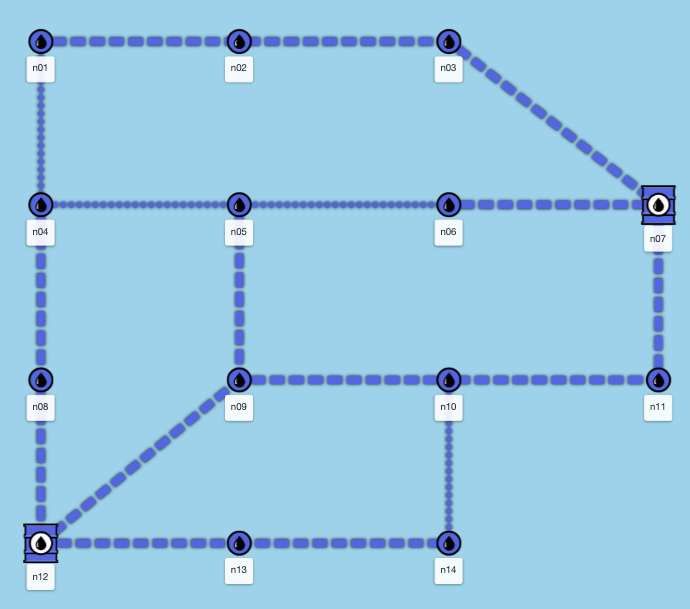
\includegraphics[width=0.6\textwidth]{images/game-graph.png}
        \caption{Game network with two supply nodes, and 12 demand nodes with "has flow", "no flow" edges.}
        \label{fig:game-graph}
    \end{figure}

    Both games simulate a fuel transportation network composed of supply nodes, demand nodes, and connecting pipelines. In \textit{Break it Bad}, the player's goal is to disrupt the network as effectively as possible using a limited number of actions. Success is measured by how much cost is inflicted on the system by strategically damaging pipelines and cutting off supply routes. In contrast, \textit{Save Our System} challenges players to preserve network stability in the face of potential disasters. Here, the goal is to mitigate risk, prepare for unpredictable events, and ensure uninterrupted fuel flow at minimal cost.

    The project aimed to:
    \begin{itemize}
        \item Build autonomous bots to play both games using rule-based strategies.
        \item Record the sequence of actions taken and the resulting scores.
        \item Analyze how different types of actions influence system performance under various conditions.
    \end{itemize}

    To achieve this, object-oriented programming principles were used to structure the bots, making them modular, extensible, and easy to test. A logging system was also developed to capture data from each gameplay session. This report details the design process, implementation logic, analysis methods, and the insights gained through experiments with different bot strategies.

\section{Game and Bot Framework}
\label{sec:game-bot-framework}
    There are a total of $10$ games that a user can play, but this semester I only worked on two of them as discussed in \cref{sec:introduction}. So, to make the project and modular bot framework extensible, I designed the codebase to be adaptable to various strategies and gameplay logic. The project is structured around a base class \texttt{DysruptionGame}, which encapsulates shared behavior such as browser login, map interaction, state inspection, and common game utilities. This base class is extended by two specialized subclasses: \texttt{BreakItBad} and \texttt{SaveOurSystem}, each implementing game-specific strategies. This design allows for easy swapping of strategies and analysis of performance data across multiple simulation runs and also makes it easy to add new games in the future for their analysis. The more details are given in \cref{sec:appendix-bot-framework}.

    \begin{figure}[h!]
        \centering
        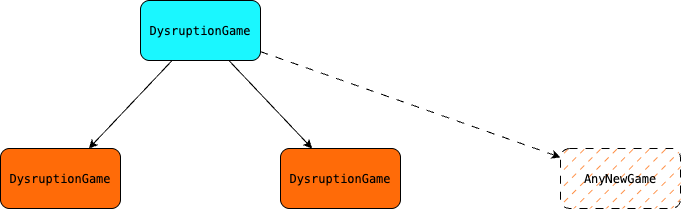
\includegraphics[width=0.8\textwidth]{images/class.png}
        \caption{Class diagram illustrating the inheritance structure of the bot framework. Any new game can be added by extending the \texttt{DysruptionGame} class.}
        \label{fig:class-diagram}
    \end{figure}

\section{Bot Action Logics}
\label{sec:bot-action-logics}
    For each game, I have given the bot a set of action logics to choose from. The bot can be configured with various decision logics, referred to as “intelligence levels” different for each games. These include:
    \begin{itemize}
        \item \textbf{Break It Bad}:
        \begin{itemize}
            \item \textbf{not\_dumb}: Will take action as a normal user, but the bot still doesn't know which action will give the highest score.
            \item \textbf{dumb}: The bot will act as dumb, meaning it can take action which a normal user will never take which will give it no boost in score.
        \end{itemize}
        
        \item \textbf{Save Our System}:
        \begin{itemize}
            \item \textbf{only\_maintain}: Only perform the maintain action on the selected edge if the bot randomly decides to take action.
            \item \textbf{only\_replace}: Only perform the replace action on the selected edge if the bot randomly decides to take action.
            \item \textbf{only\_repair}: Only perform the repair action on the selected edge if the bot randomly decides to take action.
            \item \textbf{weighted\_random}: If the bot randomly decides to take action, then if edge's:
                \begin{itemize}
                    \item FCI \(\geq 99.6\) and the cost of maintaining it is within the budget, perform the maintain action
                    \item \(92 \leq \) FCI \(< 99.6\) and the cost of repairing it is within the budget, perform the repair action
                    \item  FCI \(< 92\) and the cost of replacing the edge is within the budget, perform the replace action
                \end{itemize} 
        \end{itemize}
    \end{itemize}  

    \begin{figure}[!htbp]
        \centering
        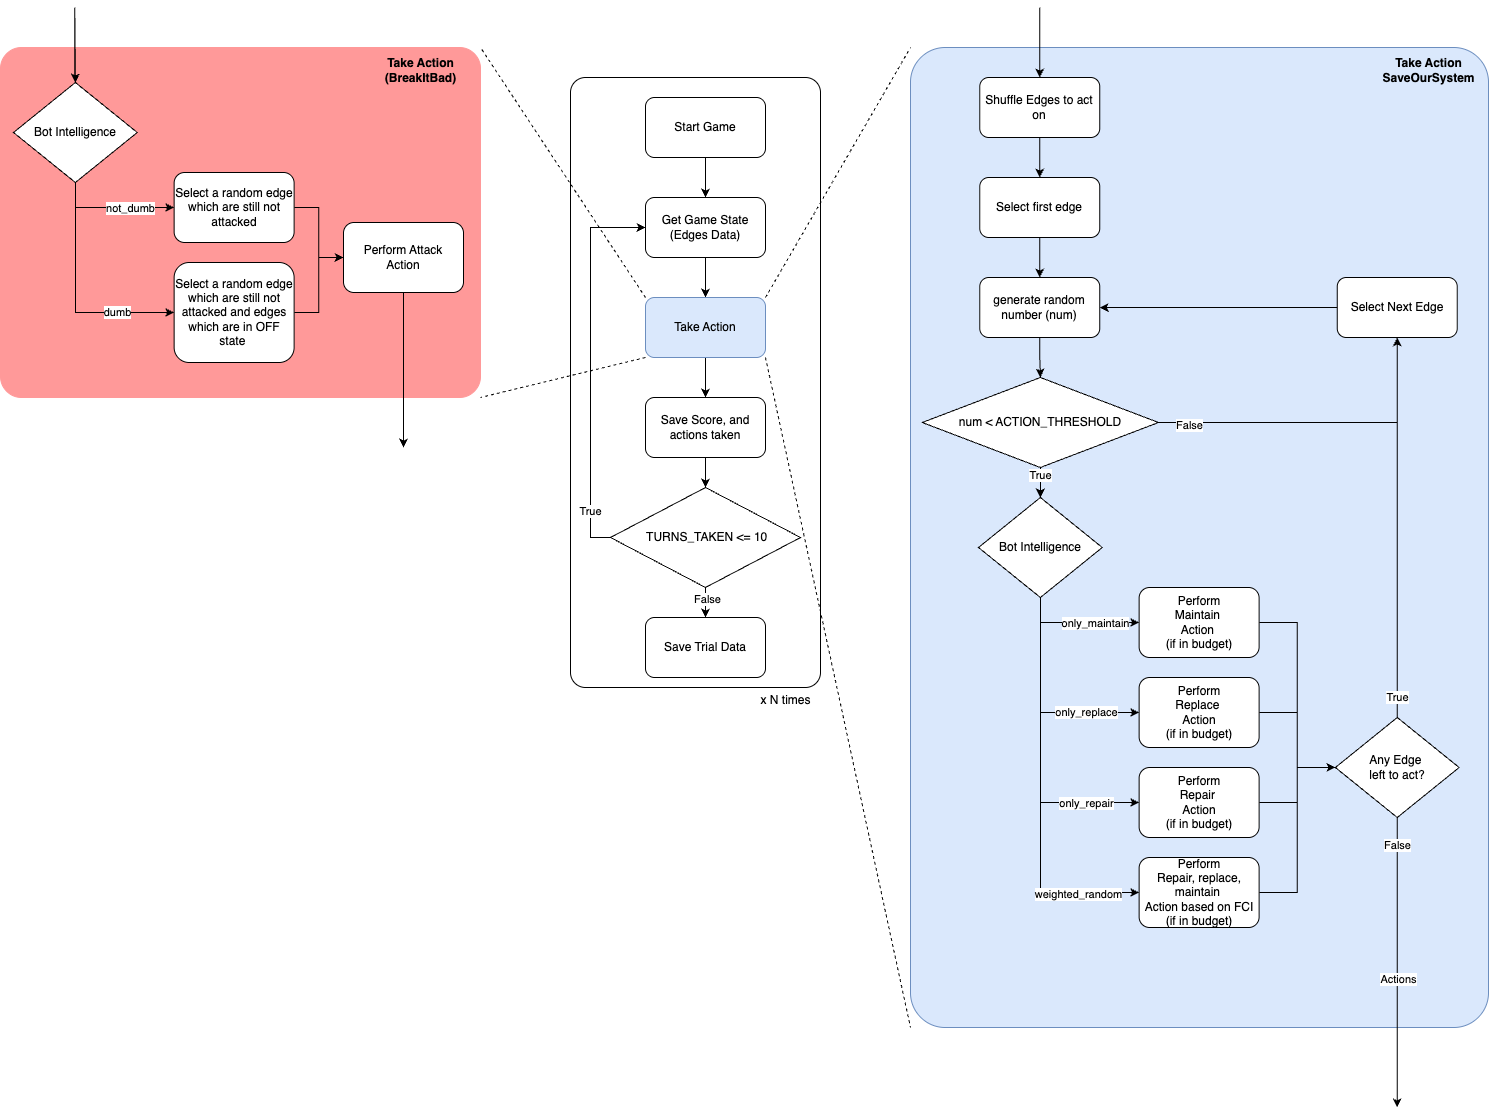
\includegraphics[width=0.8\textheight, angle=90]{images/bot-logic.png}
        \caption{Flowchart illustrating the decision-making logic of the bots for both games. The center white box is implemented in the \texttt{bot.py} and \texttt{bot-savepursystem.py} files. The other two boxes are implemented in their respective game classes in \texttt{src/game.py}.}
        \label{fig:bot-logic}
    \end{figure}

    \section{Result and Analysis}
    \label{sec:score-analysis}
        \subsection{Break It Bad}

        To evaluate the performance of the bot in the \textit{Break It Bad} game, I ran the bot in \texttt{not\_dumb} intelligence mode for approximately 500 game simulations. In each simulation, the bot executed a series of up to 5 moves, and after every move, the resulting score was recorded. The goal was to analyze how the score evolved with each action and to identify the move sequences that led to the highest disruption scores. 

        \begin{figure}[h!]
            \centering
            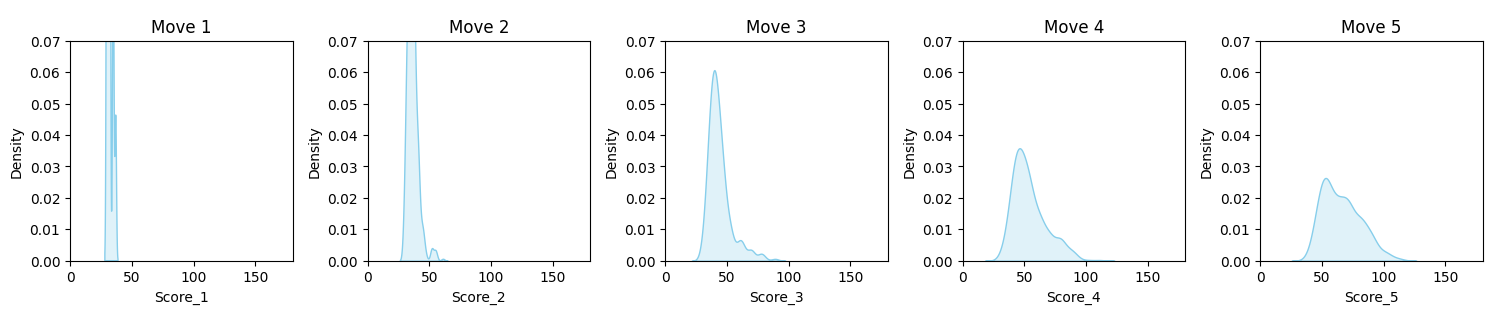
\includegraphics[width=\textwidth]{images/kde-breakitbad.png}
            \caption{KDE plot showing the distribution of scores after each move over 500 simulations (max 5 moves shown). Higher density towards the right indicates increasing score trends.}
            \label{fig:kde-breakitbad}
        \end{figure}

        As shown in \cref{fig:kde-breakitbad}, the KDE plots illustrate how the score distribution evolves with each move. Initially, the scores are tightly concentrated, but as the game progresses, the curves broaden and shift toward higher values, indicating increasing disruption. By Move 4 and Move 5, the distributions become noticeably wider and begin to exhibit bi-modal characteristics.

        To further understand the bot's decision-making, I extracted the sequence of moves that led to the highest score after 5 moves. The maximum score achieved was \textbf{113}. The corresponding sequence of moves is reported in \cref{tab:breakitbad-moves}. Each entry in the table represents an edge that was attacked during the game. The edges are represented as pairs of nodes, indicating the connections that were targeted.

        \begin{table}[h!]
            \centering
            \begin{tabular}{cc}
            \toprule
            \textbf{Move} & \textbf{Edge Attacked} \\
            \midrule
            1 & \texttt{7 <-> 3} \\
            2 & \texttt{12 <-> 8} \\
            3 & \texttt{7 <-> 6} \\
            4 & \texttt{11 <-> 7} \\
            5 & \texttt{5 <-> 9} \\
            \bottomrule
            \end{tabular}
            \caption{Sequence of moves leading to the highest score in \textit{Break It Bad}. Here, each entry \texttt{x <-> y} represents an attack on the pipeline (edge) connecting node \texttt{x} to node \texttt{y}.}
            \label{tab:breakitbad-moves}
        \end{table}

        % These results highlight that certain edge combinations consistently resulted in greater disruption and provide insight into which parts of the network are most vulnerable when targeted early.
        \subsection{Save Our System}
        To evaluate different bot strategies in the \textit{Save Our System} game, I tested all four intelligence levels from \cref{sec:bot-action-logics}, with approximately 20 trials for each and the bot’s actions and resulting scores were recorded after each game step. The best scores for each strategy are reported in \cref{tab:strategy-comparison}. Then the results of all the scenario is aggregated and analyzed and I identified the best-performing strategy based on the highest final score achieved.

        \begin{table}
            \centering
            \begin{tabular}{lc}
                \toprule
                \textbf{Strategy} & \textbf{Max Score Achieved} \\
                \midrule
                only\_maintain & 19 \\
                only\_repair & 15 \\
                only\_replace & 20 \\
                \textbf{weighted\_random} & \textbf{22} \\
                \bottomrule
            \end{tabular}
            \caption{Summary of maximum scores achieved by different strategies in the \textit{Save Our System} game.}
            \label{tab:strategy-comparison}
        \end{table}

        \begin{table}
            \centering
            \begin{tabular}{ccp{12cm}}
            \toprule
            \textbf{Move} & \textbf{Score} & \textbf{Actions Taken} \\
            \midrule
            1 & 3 & MAINTAIN: 11\texttt{$\leftrightarrow$}7, 6\texttt{$\leftrightarrow$}5, 14\texttt{$\leftrightarrow$}13, 2\texttt{$\leftrightarrow$}1, 5\texttt{$\leftrightarrow$}9, 4\texttt{$\leftrightarrow$}1, 12\texttt{$\leftrightarrow$}8, 10\texttt{$\leftrightarrow$}14 \\
            2 & 6 & MAINTAIN: 5\texttt{$\leftrightarrow$}9, 14\texttt{$\leftrightarrow$}13, 13\texttt{$\leftrightarrow$}12, 9\texttt{$\leftrightarrow$}10, 4\texttt{$\leftrightarrow$}1 \\
            3 & 7 & MAINTAIN: 9\texttt{$\leftrightarrow$}12, 10\texttt{$\leftrightarrow$}14, 4\texttt{$\leftrightarrow$}1 \\
            4 & 10 & REPAIR: 7\texttt{$\leftrightarrow$}3, REPLACE: 12\texttt{$\leftrightarrow$}8, MAINTAIN: 9\texttt{$\leftrightarrow$}10, 10\texttt{$\leftrightarrow$}14, 14\texttt{$\leftrightarrow$}13, 6\texttt{$\leftrightarrow$}5 \\
            5 & 11 & MAINTAIN: 10\texttt{$\leftrightarrow$}14, 14\texttt{$\leftrightarrow$}13, REPAIR: 7\texttt{$\leftrightarrow$}3 \\
            6 & 14 & REPLACE: 11\texttt{$\leftrightarrow$}7, MAINTAIN: 10\texttt{$\leftrightarrow$}14, REPAIR: 8\texttt{$\leftrightarrow$}4 \\
            7 & 17 & REPAIR: 5\texttt{$\leftrightarrow$}9, 2\texttt{$\leftrightarrow$}1, MAINTAIN: 10\texttt{$\leftrightarrow$}14 \\
            8 & 20 & MAINTAIN: 10\texttt{$\leftrightarrow$}14, REPLACE: 14\texttt{$\leftrightarrow$}13, REPAIR: 2\texttt{$\leftrightarrow$}3 \\
            9 & 21 & REPAIR: 2\texttt{$\leftrightarrow$}1, REPAIR: 7\texttt{$\leftrightarrow$}3 \\
            10 & 22 & REPAIR: 6\texttt{$\leftrightarrow$}5, 9\texttt{$\leftrightarrow$}12, MAINTAIN: 14\texttt{$\leftrightarrow$}13, 10\texttt{$\leftrightarrow$}14, REPAIR: 12\texttt{$\leftrightarrow$}8 \\
            \bottomrule
            \end{tabular}
            \caption{Score Progression of Best Trial for \textit{Save Our System} Game. The table shows the score after each move and the actions taken. The actions are categorized as MAINTAIN, REPAIR, or REPLACE. Here, each entry \texttt{x <-> y} represents an attack on the pipeline (edge) connecting node \texttt{x} to node \texttt{y}.}
            \label{tab:score-progression}
        \end{table}

        \Cref{tab:score-progression} highlights how the best move in \texttt{weighted\_random} strategy progressively improved the score with a balanced mix of maintenance, repair, and replacement actions. The score increase aligns with strategically targeting weakened or high-impact pipelines, showcasing this strategy’s adaptability.


    \section{Conclusion and Future Work}
    \label{sec:conclusion-future-work}
        To conclude, the project was a great learning experience in which I have created a bot framework that can be further extended to add more games in the future, if needed. For this semester the development of BreakItBad and SaveOurSystem game bots is complete and they are working as expected. The bots were able to play the games with different strategies and intelligence level as per the given requirements.

        For future work, The SaveOurSystem game bot can be improved to get more information about the best moves to make. This can be done by using reinforcement learning. Using this approach, we don't have to device the strategy for the bot like "only\_maintain", "only\_replace", etc. The bot will keep on playing the games, and will explore each and every move. After every iteration the bot will learn which move will give him best reward. After several hundred iterations, the bot will learn the best policy to play the game and then we can judge the bot which action to take. This approach will be best for this game as the this game environment is random, and to get fruitful results, we don't have to define the strategy for the bot but let the bot explore the game and learn from it.

\section{Acknowledgements}
    \label{sec:acknowledgements}
    I would like to thank Dr. Thomas Seager for giving me an opportunity to assist in his research project. His guidance and inputs helped shape the direction of the work and ensured its successful completion. I would also like to thank Mazin Abdel Magid for explaining the project and it's requirements in detail.

    \clearpage
% Removed \newpage as it is unnecessary or misplaced
\section*{Appendix}
\addcontentsline{toc}{section}{Appendix}
\appendix
    \section{Repository Structure}
    Here I will give the structure of the repository and a brief description of each file and folder. And how to use, and where make changes if needed.

    \dirtree{%
        .1 /.
        .2 config.
        .3 breakitbad.py.
        .3 saveoursystem1.py.
        .2 src.
        .3 game.py.
        .3 utils.
        .4 const.py.
        .4 Edge.py.
        .4 metrics.py.
        .4 Node.py.
        .2 bot.py.
        .2 bot-saveoursystem.py.
        .2 requirements.txt.
    }

    \vspace{1cm}
    The details of the files and folders are as follows:

    \begin{itemize}
        \item \textbf{config/}: Contains the configuration files for each game that the bot reads. It contains some settings that the bot needs to run. Each game have its own configuration file. In this the user can change number of trials to run, the game URL, and the bot's intelligence level.
            \begin{itemize}
                \item \texttt{break\_it\_bad.py}: Configuration file for the \texttt{BreakItBad} game.
                \item \texttt{save\_our\_system.py}: Configuration file for the \texttt{SaveOurSystem} game.
            \end{itemize}
        \item \textbf{src/}: Source code for the bot framework and game-specific implementations.
            \begin{itemize}
                \item \texttt{game.py}: This is main game file where the base game class and BreakItBad, SaveOurSystem derived game classes are defined. If any new game needs to be added, it can be added in this file.
                \item \texttt{utils/}: This folder contains the utility files like data classes to save Node and Edges data, and some constants used in game.
            \end{itemize}
        \item \textbf{bot.py}: The bot file for BreakItBad game. To run this game simply run it in ternminal using \texttt{python3 bot.py} command.
        \item \textbf{bot-saveoursystem.py}: The bot file for BreakItBad game. To run this game simply run it in ternminal using \texttt{python3 bot-saveoursystem.py} command.
        \item \texttt{requirements.txt}: List of Python dependencies required to run the project. It can be used to create python environment for this project.
    \end{itemize}


    \section{Detailed Bot Framework Design}
    \label{sec:appendix-bot-framework}

    \subsection*{Class Design}
    \label{subsec:class-design}

    The codebase is centered around a base class \texttt{DysruptionGame}, which encapsulates shared behavior such as browser login, map interaction, state inspection, and common game utilities. This base class is extended by two specialized subclasses:
    \begin{itemize}
        \item \texttt{BreakItBad}: Implements logic to attack pipelines and maximize disruption.
        \item \texttt{SaveOurSystem}: Focuses on maintenance and repair actions under a constrained budget.
    \end{itemize}

    Each subclass overrides and extends the behavior of the base class to implement game-specific strategies, including action selection and score retrieval.

    \subsection*{Class: DysruptionGame}
    \label{subsec:class-dysruptiongame}

    The \texttt{DysruptionGame} class serves as the foundational blueprint for automating interactions with the simulation games. It abstracts repetitive tasks such as navigating the game UI, extracting map state, and performing actions. Below is a summary of its core components and functions:

    \begin{itemize}
        \item \textbf{Constructor (\_\_init\_\_)}: Initializes the game by setting the URL, intelligence strategy, and configuration flags. It also launches the game and prepares the node/edge storage.
        
        \item \textbf{reset\_game(first\_run=False)}: Opens the game in a browser and waits for key UI elements to load. If it's the first run, it waits for the login prompt; otherwise, it waits for the intro banner.

        \item \textbf{initiliaze\_edges\_nodes()}: Initializes empty lists to hold node and edge objects before parsing the game state.

        \item \textbf{login()}: Fills in the username field and submits the login form to enter the game environment.

        \item \textbf{start\_game()}: Waits for the intro banner and map buttons to load, then clicks through to start the game.

        \item \textbf{activate\_map\_read\_mode()}: Enables read mode by clicking the map selector, which allows edge and node information to be read.

        \item \textbf{find\_edges()}: Finds all visible pipeline edges on the map and reads their visual properties (e.g., flow direction and status) to initialize them as \texttt{Edge} objects.

        \item \textbf{find\_edges\_state()}: Clicks each edge to extract additional metadata from the inspector panel such as temperature, flow, and FCI (Failure Condition Index).

        \item \textbf{find\_nodes()}: Detects all nodes on the map and classifies them as supply or demand based on visual styles.

        \item \textbf{find\_nodes\_state()}: Extracts detailed data for each node (like name, penalty, demand, or shortfall) by reading the inspector panel.

        \item \textbf{random\_action()}: Returns \texttt{True} or \texttt{False} based on a threshold probability. Useful for making bots act probabilistically.

        \item \textbf{action()}: Waits for the game’s UI to be ready before allowing the next action. Used to introduce pacing between bot moves.

        \item \textbf{quit()}: Shuts down the browser session cleanly.
    \end{itemize}

    By consolidating this core functionality, the class serves as a reliable and reusable foundation for building bots for multiple games.


    \subsection*{Class: BreakItBad}
    \label{subsec:class-breakitbad}

        The \texttt{BreakItBad} class extends the base \texttt{DysruptionGame} class to implement logic specific to the "Break it Bad" game scenario. In this game, the objective is to disrupt the fuel distribution network as much as possible within a limited number of moves.

        Key components of the class include:

        \begin{itemize}
            \item \textbf{Constructor (\_\_init\_\_)}: Initializes the inherited attributes and settings for the BreakItBad game.

            \item \textbf{initiliaze\_edges\_nodes()}: Overrides the base method to additionally prepare separate lists for attacked, not attacked, and off-state edges.

            \item \textbf{get\_score()}: Extracts the current score from the scoreboard element on the page using Selenium.

            \item \textbf{attack()}: Depending on the selected intelligence strategy, chooses an edge to attack—either randomly or selectively—and executes a simulated click on it.

            \item \textbf{action()}: Executes an attack via the \texttt{attack()} function and then calls the base class's \texttt{action()} method to continue the game loop.

            \item \textbf{is\_game\_over()}: Checks whether the game is complete by verifying if all available attackable edges have been used.

            \item \textbf{filter\_edges()}: Sorts all edges into categories (not attacked, stopped, attacked) based on their current status for better decision-making.

            \item \textbf{deactivate\_map\_read\_mode()}: Switches off map read mode and enables attack mode by clicking the corresponding UI button.

            \item \textbf{get\_state()}: Combines all logic to refresh the current map state, including reading nodes, edges, and their properties. Includes retries to ensure robustness.
        \end{itemize}

        This class encapsulates all behavior specific to the BreakItBad game and provides a structured approach to implementing bot behavior for disruptive gameplay.


    \subsection*{Class: SaveOurSystem}
    \label{subsec:class-saveoursystem}

        The \texttt{SaveOurSystem} class is a subclass of \texttt{DysruptionGame} and implements logic for the defensive gameplay scenario, where the player must maintain and restore a critical fuel network under a constrained budget. It includes multiple types of actions—repair, replace, and maintain—each with different costs and effects.

        Key components of the class include:

        \begin{itemize}
            \item \textbf{Constructor (\_\_init\_\_)}: Inherits all base parameters and initializes edge categories for this game.

            \item \textbf{initiliaze\_edges\_nodes()}: Extends the base method to additionally set up lists for operational and destroyed edges.

            \item \textbf{get\_score()}: Extracts the current performance score displayed in the game.

            \item \textbf{get\_budget()}: Reads the current available budget from the game UI, which is needed to decide on allowable actions.

            \item \textbf{perform\_action(edge, action\_button\_selector)}: Clicks the appropriate repair, replace, or maintain button, then applies the action on the selected edge.

            \item \textbf{action()}: Implements strategy-specific logic. Depending on the intelligence mode, the bot chooses which action to perform while staying within the budget. The \texttt{weighted\_random} mode evaluates edge health (FCI) before deciding.

            \item \textbf{is\_game\_over()}: Placeholder check for game-ending condition (inherited from base), though not directly tied to game logic in this case.

            \item \textbf{filter\_edges()}: Classifies edges as destroyed or operational based on their failure index, used to prioritize repairs.

            \item \textbf{get\_state()}: Aggregates all state-gathering steps: node and edge detection, edge detail extraction, and classification.
        \end{itemize}

        This class enables simulation of different maintenance strategies and their effectiveness in keeping the network operational despite failures and budget constraints.
    
    \subsection*{bot.py and bot-saveoursystem.py}
    \label{subsec:bot-files}

        The \texttt{bot.py} and \texttt{bot-saveoursystem.py} files serve as the entry points for running the bots in their respective games. They create the objects of game classes, and execute the main game loop. The main loop can be visualized in the \cref{fig:bot-logic} flowchart in the center white box.
    
    \section{How to Run the Project}
    \label{sec:how-to-run}
    To run the project, follow these steps:
    \begin{itemize}
        \item Clone the repository to your local machine.
        \item Navigate to the project directory.
        \item Download chromedriver and place it in the same directory as the project, and update config/breakitbad.py and config/saveoursystem1.py files with the path to the chromedriver.
        \item Install the required dependencies using:
            \begin{verbatim}
                pip install -r requirements.txt
            \end{verbatim}
        \item Change the configuration files in the \texttt{config} folder as per your requirements. The configuration files are:
            \begin{itemize}
                \item \texttt{break\_it\_bad.py}: Configuration file for the \texttt{BreakItBad} game.
                \item \texttt{save\_our\_system.py}: Configuration file for the \texttt{SaveOurSystem} game.
            \end{itemize}
        \item Run the bot for the desired game:
            \begin{verbatim}
                python3 bot.py
            \end{verbatim}
            or
            \begin{verbatim}
                python3 bot-saveoursystem.py
            \end{verbatim}
    \end{itemize}
        
\end{document}